\clearpage

\section {Predictions of single $\mu$-like ring event reconstructed energy spectrum in SuperK}
\label{sec:spectrum_prediction}

\subsection {Methodology}

In this analysis, 
the oscillation parameters are determined 
by fitting the reconstructed energy ($E_{r}$) spectrum
of 1 $\mu$-like ring events observed at SuperK with the predicted spectrum.
The predicted number $N_{SK;r}$ 
of 1 $\mu$-like ring events in the $r^{th}$ reconstructed energy bin
is computed as follows:

\begin{equation}
\displaystyle
  N_{SK;r} = 
    \sum_{m} \sum_{t} \sum_{r\prime}
        P_{m;t} \cdot
        T_{r;r\prime;f_{E; r}^{SK}} \cdot
        S_{m;t;r\prime;\vec{f}} \cdot
        N_{SK;m;r\prime;t}^{MC} \cdot
\label{eq:far_prediction}
\end{equation}

In Eq.\ \ref{eq:far_prediction}, $N_{SK;m;r\prime;t}^{MC}$ is the input SuperK Monte Carlo (MC) template 
containing the number of events in the 1 $\mu$-like ring MC sample with true reaction mode $m$ in the 
true energy bin t and the reconstructed energy bin $r\prime$.
The construction of the nominal MC templates is discussed in Sec.\ \ref{sec:mc_templates}.
Both flux-tuning weights based on NA61 hadron-production data (see Sec.\ \ref{sec:na61_weights})
and flux and cross-section tuning weights based on ND280 data (see Sec.\ \ref{sec:banff_weights})
are applied to the nominal MC templates.
$S_{m;t;r\prime;\vec{f}}$ is an overall, multiplicative, systematic error factor 
depending on the reaction mode $m$, the true energy bin $t$, the reconstructed energy bin $r\prime$ 
and a vector of nuisance (systematic) parameters $\vec{f}$. 
A complete description of the nuisance parameters considered in this analysis is given in Sec.\ \ref{sec:systematics}.
$T_{r;r\prime;f_{E; r}^{SK}}$ is a transfer function describing the migration of events
between the reconstructed energy bins $r$ and $r\prime$ due to uncertainty in the SuperK reconstructed energy
scale, expressed here in terms of the nuisance parameter $f_{E; r}^{SK}$.
Finally, $P_{m;t}$ is the 3-flavour oscillation probability applied to the true energy
bin t of the SuperK MC template which corresponds to mode $m$;
application of the term $P_{m;t}$ is discussed in Sec.\ \ref{sec:applying_oscillations}.

%....................................................................................................................
%....................................................................................................................

\subsection {Construction of nominal SuperK Monte Carlo templates}
\label{sec:mc_templates}

The nominal SuperK 1 $\mu$-like ring MC templates $N_{SK;m;r;t}^{MC}$
are constructed by applying the 1 $\mu$-like ring selection cuts to the official SuperK MC samples.
Details of the MC samples are given in Sec.\ \ref{sec:mc_templates:input_mc}.
The calculation of the normalization of each MC sample is described in Sec.\ \ref{sec:mc_templates:normalization}.
The official 1 $\mu$-like ring selection cuts are listed in Sec.\ \ref{sec:mc_templates:1Rmu_cuts}.
The list of MC templates used in this analysis is shown in Sec.\ \ref{sec:mc_templates:template_list},
while the true and reconstructed energy binning of the templates is discussed 
in Sec.\ \ref{sec:mc_templates:template_binning}.
The nominal SuperK MC templates used in this analysis are shown in \cite{OurRun1234DisappAnalysisSupplement}.

%....................................................................................................................
\subsubsection {Input Monte Carlo samples}
\label{sec:mc_templates:input_mc}

This analysis uses the official 2013a SuperK MC samples generated using the 11btunedv3.2 JNUBEAM flux.
Five MC samples were generated.
Four of the samples
($\nu_{\mu}$, $\bar{\nu}_{\mu}$, $\nu_{e}$ and $\bar{\nu}_{e}$) 
were generated using the nominal JNUBEAM flux without oscillations.
A fifth sample of $\nu_{e}$ interactions was also generated with the $\nu_{\mu}$ flux.
This fifth sample will be denoted the ``oscillated $\nu_{e}$'' sample (it corresponds to the ``signal-$\nu_{e}$'' 
sample in the $\nu_{e}$-appearance analysis).
For completeness, we added four new samples compared with our Run 1+2+3 analysis, and these are oscillated $\nu_{e} \rightarrow \nu_{\mu}$ CCQE, 
oscillated $\nu_{e} \rightarrow \nu_{\mu}$ CC1$\pi$, oscillated $\nu_{e} \rightarrow \nu_{\mu}$ CC coherent and 
oscillated $\nu_{e} \rightarrow \nu_{\mu}$ CC other. Since a separate official oscillated $\nu_{e} \rightarrow \nu_{\mu}$ 
SuperK sample is not available, we emulated it by reweighting the $\nu_\mu$ SuperK MC sample with the $\nu_e$ flux
(the oscillated $\nu_{e} \rightarrow \nu_{\mu}$ are not statistically independent of the $\nu_\mu$ templates).
All samples were generated including the neutrino flux estimates up to 30 GeV.
The flux histograms used for neutrino event generation had 50 MeV bins.

%....................................................................................................................
\subsubsection {Normalization of Monte Carlo samples}
\label{sec:mc_templates:normalization}

The normalization (integrated exposure in terms of POT) of each event sample is calculated from
the number of events with a MC truth interaction vertex within the 22.5 kt fiducial volume.

\begin{equation}
\displaystyle
  N = \int  dS dI dE \cdot
            \frac{d^{3}\Phi_{SK}}{dS dI dE_{\nu}} \cdot
            \sigma_{H_{2}O} \cdot
            \frac{N_{A}}{A} \cdot \rho \cdot L 
\end{equation}
where 
$d^{3}\Phi_{SK}$/$dS dI dE$ is the number of flux particles for the given neutrino species 
per neutrino energy bin $dE_{\nu}$, per unit area $dS$ and per POT,
$\sigma_{H_{2}O}$ is the total interaction cross section in water
for the given neutrino species,
I is the beam intensity in terms of POT,
$N_{A}$ is  Avogadro's number,
$A$ is the mass number for water,
$\rho$ is the water density
and L is the neutrino path length in the water volume.
%The results of this calculation are shown in Tab.\ \ref{tab:SKMCSummary} for all 5 SuperK MC samples along with 
%the generated statistics, the numbers of events within the 22.5 kt fiducial volume and the
%derived POT normalization of each sample in terms of POT.
The derived POT normalization of each sample is shown in Tab.\ \ref{tab:SKMCSummary}.
After being generated from a MC sample corresponding to a calculated integrated beam exposure I,
each MC template is normalized to the integrated beam exposure of the Run 1+2+3+4 dataset (6.5700$\times$10$^{20}$ POT)
by scaling the bin contents of the template with 6.5700$\times$10$^{20}$/I.

\begin{table}
\centering
% \begin{tabular}{| c | c | c | c | c |}
% \hline
% Sample             &  Number of events   &  Number of events  & Number of events  & POT normalization \\
%                    & /22.5 kt fiducial /$10^{21}$ POT  & generated  & in fiducial volume  &               \\  
% \hline             
% $\nu_{\mu}$            &          &            &             &     x.xxxx $\times 10^{2?}$  \\
% $\bar{\nu_{\mu}}$      &          &            &             &     x.xxxx $\times 10^{2?}$ \\
% $\nu_{e}$              &          &            &             &     x.xxxx $\times 10^{2?}$ \\
% $\bar{\nu_{e}}$        &          &            &             &     x.xxxx $\times 10^{2?}$ \\
% Oscillated $\nu_{e}$   &          &            &             &     x.xxxx $\times 10^{2?}$ \\
\begin{tabular}{| c | c |}
\hline
Sample             &  POT normalization \\
\hline             
$\nu_{\mu}$            & 4.47598 $\times 10^{23}$ \\
$\bar{\nu}_{\mu}$      & 6.57643 $\times 10^{24}$ \\
$\nu_{e}$              & 2.23833 $\times 10^{25}$ \\
$\bar{\nu}_{e}$        & 1.06961 $\times 10^{26}$ \\
Oscillated $\nu_{e}$   & 2.14913 $\times 10^{23}$ \\
\hline
\end{tabular}
\caption{
  Normalization of input SuperK MC samples.
  %Statistics and normalization of input SuperK MC samples.
}
\label{tab:SKMCSummary}
\end{table}

%....................................................................................................................
\subsubsection {Single $\mu$-like ring event selection cuts}
\label{sec:mc_templates:1Rmu_cuts}

The SuperK MC templates contain events from the 
$\nu_{\mu}$, $\bar{\nu}_{\mu}$, $\nu_{e}$, $\bar{\nu}_{e}$, oscillated $\nu_{e}$ and oscillated $\nu_{\mu}$ samples
passing the standard SuperK selection cuts for 1 $\mu$-like ring events.
These cuts are:

\begin{itemize}
\item
the number of PMT hits in the highest-charge OD cluster is less than or
equal to 15, and the event passes the flasher rejection cuts
({\tt evclass == 1}),
\item
the reconstructed vertex is at least 2 metres away from the ID wall 
({\tt wall $>$ 200}),
\item
the visible energy in the event is above 30 MeV 
({\tt evis  $>$ 30}),
\item
there is exactly 1 reconstructed ring in the event 
({\tt nring == 1}),
\item
the reconstructed ring is $\mu$-like 
({\tt ip[0] = 3}),
\item
the reconstructed muon momentum is above 200 MeV 
({\tt amomm[0] $>$ 200}), and
\item
there is at most 1 decay e$^{-}$ in the event 
({\tt nmue $<$= 1}).
\end{itemize}

%....................................................................................................................
\subsubsection {List of Monte Carlo templates}
\label{sec:mc_templates:template_list}

For each SuperK MC sample, a number of different MC templates is constructed 
corresponding to different true reaction modes.
The template granularity depends on the type of oscillation analysis and the specific 
systematic parameters considered in the analysis.
12 MC templates were used for our 2010 Run 1+2 2-flavour disappearance analysis \cite{OurRun12DisappAnalysis}, while
15 MC templates were used for our 2010 Run 1+2 3-flavour disappearance analysis \cite{OurRun12DisappAnalysis3Flavour} and
28 MC templates were used for our 2012 Run 1+2+3 3-flavour disappearance analysis \cite{OurRun123DisappAnalysis3Flavour}.
This analysis uses the following 32 MC templates:

\begin{itemize}
\item  $\nu_{\mu}$ CCQE
\item  $\nu_{\mu}$ CC1$\pi$, 
\item  $\nu_{\mu}$ CC coherent, 
\item  $\nu_{\mu}$ CC other, 
\item  $\nu_{\mu}$ (and $\rightarrow$ $\nu_{e}$, $\nu_{\tau}$) NC1$\pi^{\pm}$, 
\item  $\nu_{\mu}$ (and $\rightarrow$ $\nu_{e}$, $\nu_{\tau}$) NC other, 
\item  $\bar{\nu}_{\mu}$ CCQE, 
\item  $\bar{\nu}_{\mu}$ CC1$\pi$, 
\item  $\bar{\nu}_{\mu}$ CC coherent, 
\item  $\bar{\nu}_{\mu}$ CC other, 
\item  $\bar{\nu}_{\mu}$(and $\rightarrow$ $\bar{\nu}_{e}$, $\bar{\nu}_{\tau}$) NC1$\pi^{\pm}$, 
\item  $\bar{\nu}_{\mu}$(and $\rightarrow$ $\bar{\nu}_{e}$, $\bar{\nu}_{\tau}$) NC other, 
\item  $\nu_{e}$ CCQE, 
\item  $\nu_{e}$ CC1$\pi$,
\item  $\nu_{e}$ CC coherent,
\item  $\nu_{e}$ CC other,
\item  $\nu_{e}$ (and $\rightarrow$ $\nu_{\mu}$, $\nu_{\tau}$) NC1$\pi^{\pm}$,
\item  $\nu_{e}$ (and $\rightarrow$ $\nu_{\mu}$, $\nu_{\tau}$) NC other,
\item  $\bar{\nu}_{e}$ CCQE, 
\item  $\bar{\nu}_{e}$ CC1$\pi$,
\item  $\bar{\nu}_{e}$ CC coherent,
\item  $\bar{\nu}_{e}$ CC other,
\item  $\bar{\nu}_{e}$ (and $\rightarrow$ $\bar{\nu}_{\mu}$, $\bar{\nu}_{\tau}$) NC1$\pi^{\pm}$,
\item  $\bar{\nu}_{e}$ (and $\rightarrow$ $\bar{\nu}_{\mu}$, $\bar{\nu}_{\tau}$) NC other,
\item  oscillated $\nu_{\mu} \rightarrow \nu_{e}$ CCQE,
\item  oscillated $\nu_{\mu} \rightarrow \nu_{e}$ CC1$\pi$,
\item  oscillated $\nu_{\mu} \rightarrow \nu_{e}$ CC coherent,
\item  oscillated $\nu_{\mu} \rightarrow \nu_{e}$ CC other,
\item  oscillated $\nu_{e} \rightarrow \nu_{\mu}$ CCQE,
\item  oscillated $\nu_{e} \rightarrow \nu_{\mu}$ CC1$\pi$,
\item  oscillated $\nu_{e} \rightarrow \nu_{\mu}$ CC coherent, and
\item  oscillated $\nu_{e} \rightarrow \nu_{\mu}$ CC other.
\end{itemize}

%....................................................................................................................
\subsubsection {Binning of Monte Carlo templates}
\label{sec:mc_templates:template_binning}

Each of the 32 MC templates has 6132 2-dimensional bins (= 84 true energy bins $\times$ 73 reconstructed energy bins).
The 84 true energy bins are arranged as follows:
\begin{itemize}
 \item   6 50-MeV bins from 0-0.3 GeV, 
 \item   28 25-MeV bins from 0.3-1 GeV, 
 \item   40 50-MeV bins from 1-3 GeV, 
 \item   5 100-MeV bin from 3-3.5 GeV, 
 \item   1 bin from 3.5-4 GeV, 
 \item   1 bin from 4-5 GeV, 
 \item   1 bin from 5-7 GeV, 
 \item   1 bin from 7-10 GeV and
 \item   1 bin from 10-30 GeV.
\end{itemize}

The 73 reconstructed energy bins are the following:
\begin{itemize}
 \item   60 50-MeV bins from 0-3 GeV, 
 \item   4 250-MeV bins from 3-4 GeV, 
 \item   4 500-MeV bins from 4-6 GeV, 
 \item   4 1000-MeV bins from 6-10 GeV and
 \item   1 bin from 10-30 GeV.
\end{itemize}
The same reconstructed neutrino energy binning is used for the fit of the 1-ring $\mu$-like reconstructed energy spectrum.

A study was performed to decide the optimum binning scheme balancing the needs for accuracy and speed.
Details are given in Appendix I of Ref.\ \cite{OurRun123DisappAnalysis3Flavour}.

The binning described here is unchanged with respect to the Run 1+2+3 analysis,
but, after discussion with T2K-SK, events with reconstructed energy $>$30 GeV are now included in
the 10-30 GeV bin.

%....................................................................................................................
%....................................................................................................................
\subsection {Applying flux tuning based on NA61 data}
\label{sec:na61_weights}

In this analysis, the nominal MC templates, which were constructed using a MC event sample generated with the 11a flux,
are reweighted to the 11bv3.2 flux which was tuned on NA61 hadron production measurements \cite{FluxTuning}\cite{NA61T2K}.
The reweighted MC templates are denoted the {\em NA61-tuned} MC templates in this document.
The applied weights were obtained from \cite{FluxTuningHistograms} and are shown as a function of the true neutrino energy 
in Figs.\ 1-4 in Ref.\ \cite{OurRun123DisappAnalysis3Flavour}.
The effect of this flux tune on the predicted reconstructed energy spectrum of 
single $\mu$-like ring events is discussed in Sec.\ \ref{sec:nominal_and_tuned_predictions} 
(see Figs.\ \ref{fig:nsk_vs_osc_params_effect_of_na61_tune} and \ref{fig:1Rmu_spectrum_w_and_wo_na61_weights}, and 
Tabs.\ \ref{tab:nsk_nominal_x3_no_osc} and \ref{tab:nsk_nominal_x3_default_osc})

%
%\begin{figure*}[htb]
%\begin{minipage}[t]{0.48\linewidth}
%\center
%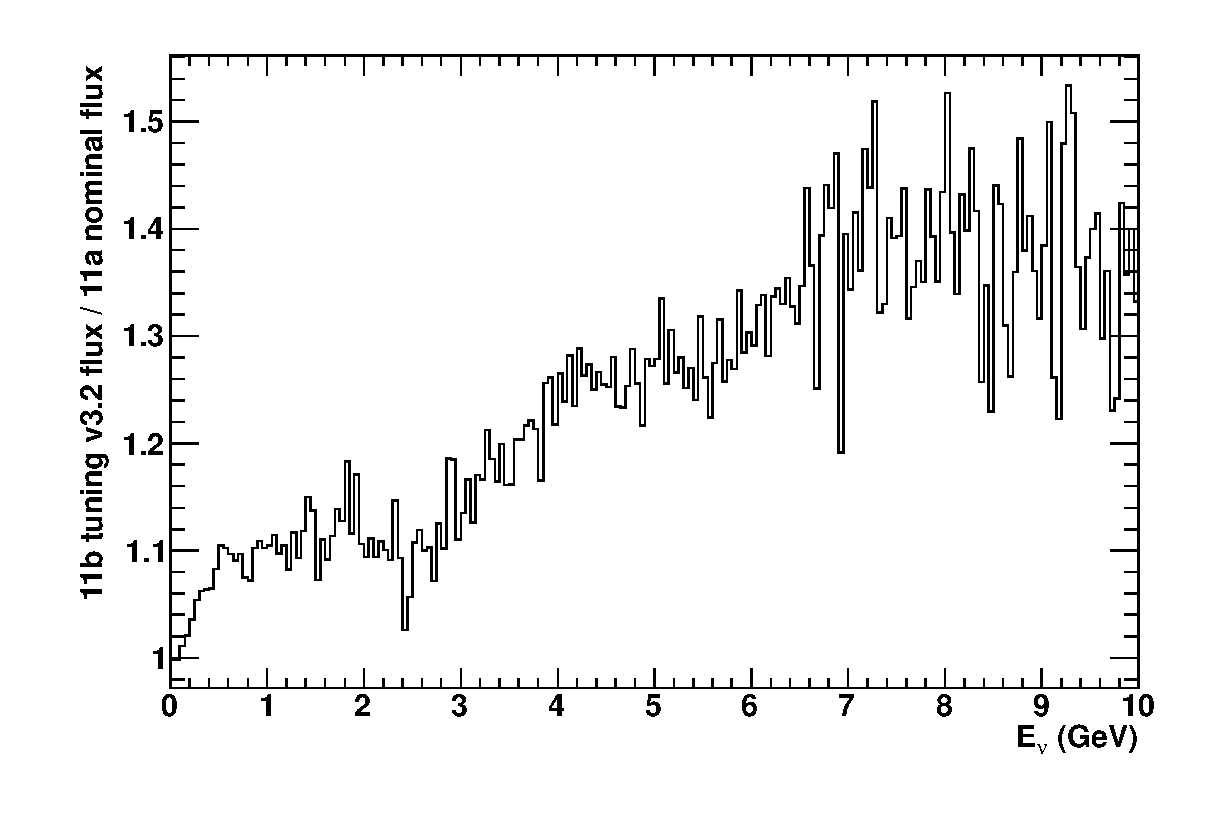
\includegraphics[width=18pc]{./images/fluxtune/fluxtune_numu}
%\caption {
%  $\nu_\mu$ 2011b\_v3.2\_run1-3c flux tuning weights applied to nominal $\nu_\mu$ and oscillated-$\nu_e$ MC templates.}
%\label{fig:na61_weights:numu}
%\end{minipage}
%\hspace{0.06\linewidth}
%\begin{minipage}[t]{0.48\linewidth}
%\center
%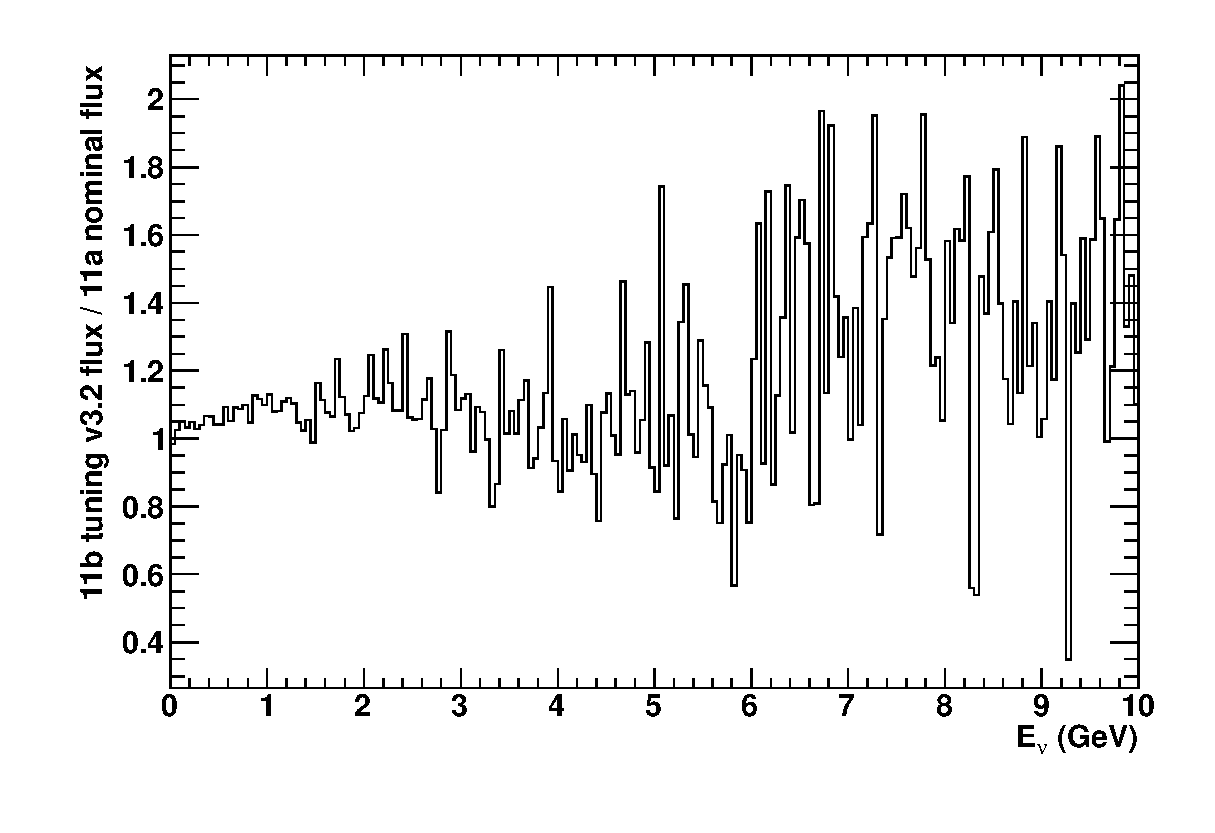
\includegraphics[width=18pc]{./images/fluxtune/fluxtune_numub}
%\caption {
%  $\bar{\nu_\mu}$ 2011b\_v3.2\_run1-3c flux tuning weights applied to nominal $\bar{\nu_\mu}$ MC templates.}
%\label{fig:na61_weights:numubar}
%\end{minipage}
%\vfill
%\begin{minipage}[t]{0.48\linewidth}
%\center
%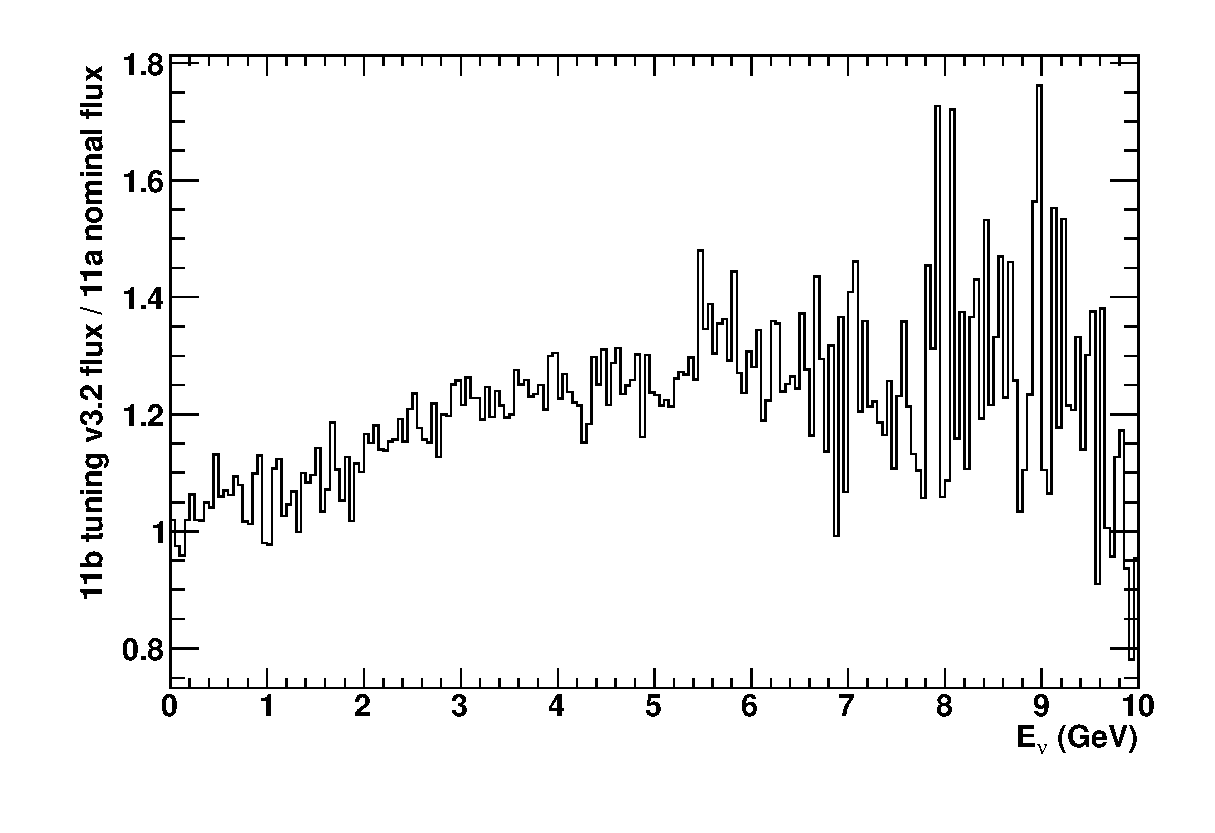
\includegraphics[width=18pc]{./images/fluxtune/fluxtune_nue}
%\caption {
%  $\nu_e$ 2011b\_v3.2\_run1-3c flux tuning weights applied to nominal $\nu_e$ MC templates.}
%\label{fig:na61_weights:nue}
%\end{minipage}
%\hspace{0.06\linewidth}
%\begin{minipage}[t]{0.48\linewidth}
%\center
%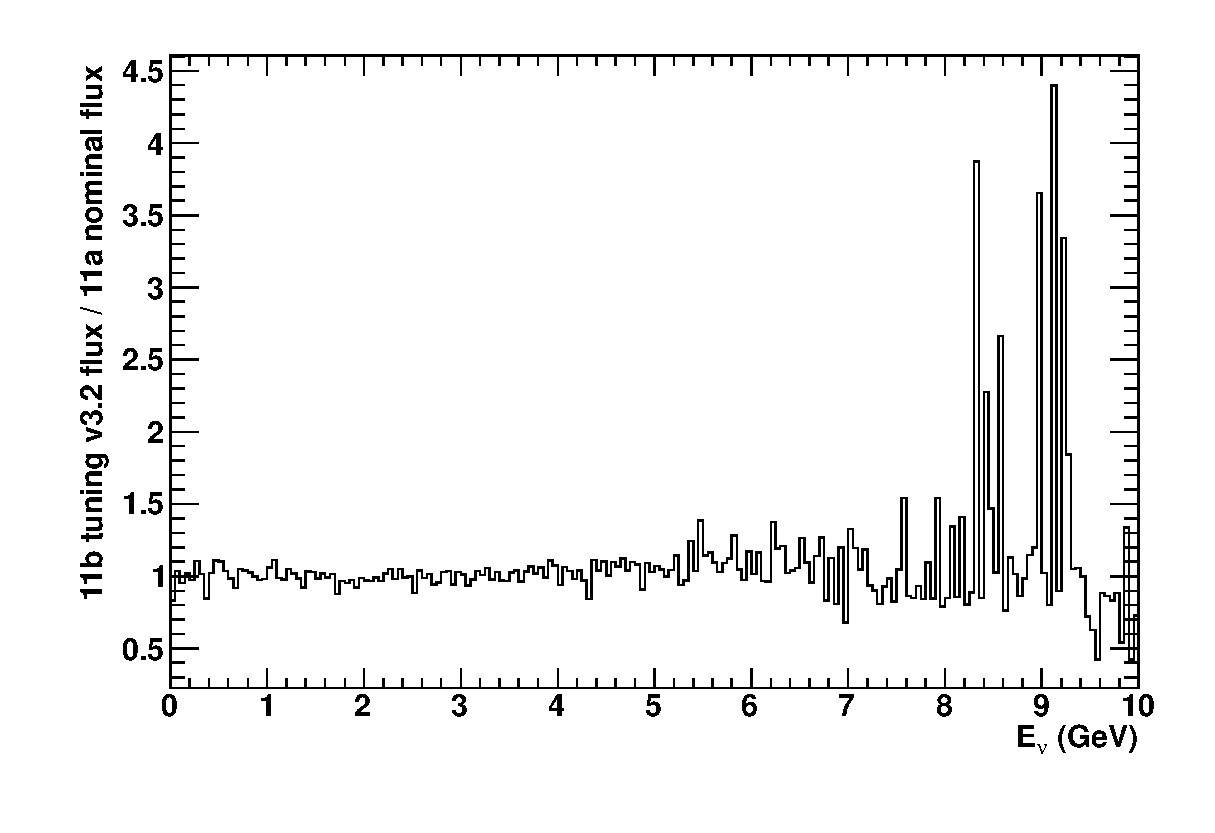
\includegraphics[width=18pc]{./images/fluxtune/fluxtune_nueb}
%\caption {
%  $\bar{\nu_e}$ 2011b\_v3.2\_run1-3c flux tuning weights applied to nominal $\bar{\nu_e}$ MC templates.}
%\label{fig:na61_weights:nuebar}
%\end{minipage}
%\end{figure*}
%

%....................................................................................................................
%....................................................................................................................

\subsection {Applying flux and cross-section (BANFF) tuning based on ND280 data}
\label{sec:banff_weights}

This analysis uses the BANFF flux and cross-section parameter tuning to reweight the NA61-tuned MC templates.
The MC templates obtained after this second reweighting will be denoted the {\em BANFF-tuned} MC templates
in this document.
Updated BANFF weights were used in this analysis with respect to the Run 1+2+3 one.

For the 2013 analyses, the ND280 $\nu_{\mu}$ group has updated the division of reconstructed ND280 CC events. 
These events are now divided into the CC0$\pi$-like, CC1$\pi$-like and CC other samples (whereas for the Run 1+2+3 analysis they were divided into CCQE-like 
and CCnonQE samples). Pion tracks are identified using ionisation energy losses in the TPC or FGD, or a pion can be identified
by the presence of a Michel electron in FGD1. The CC0$\pi$-like and CC1$\pi$-like samples have exactly 0 and 1 track consistent with
a $\pi^{+}$ respectively. The CC other sample consists of events with more than 1 track consistent with a $\pi^{+}$ or at least
one negative track or with a track consistent with an electron \cite{ND280Inputs}. The BANFF group has made a fit of these three ND280 
samples to find the best-fit values of the flux normalisation parameters and the cross-section parameters whose errors are expected to 
have some cancellation between the ND280 and SuperK, and the correlations between these parameters \cite{BANFF2013}. The postfit values of these 
parameters (taken from version 5 of the 2013 Run 1+2+3+4 BANFF fit in \verb+postfit_banff_2013_disappearance_v5.root+) are used in
turn to calculate the nominal predicted single $\mu$-like ring reconstructed energy spectrum in SuperK.
A list of BANFF parameters and their best-fit values is shown in Tab.\ \ref{tab:input_uncertainties}.

%This analysis reweights the NA61-tuned MC templates to the BANFF best-fit parameters
%\footnote{
%  The BANFF group performed its fit using an NA61-tuned flux ({\em 2011b\_v3.2\_run1-3c}),
%  the same one used for reweighting our nominal MC templates in Sec.\ \ref{sec:na61_weights}.
%}
%\footnote{
%  Reweighting the MC templates to the BANFF best-fit parameters is, in effect, a ``special''
%  systematic variation. Therefore, more details on 
%  are presented in the section detailing the systematic parameters considered in this analysis
%  (Sec.\ \ref{sec:systematics}).
%}.

The effect of the BANFF tune on the predicted reconstructed energy spectrum of
single $\mu$-like ring events is discussed in Sec.\ \ref{sec:nominal_and_tuned_predictions} (see 
Figs.\ \ref{fig:nsk_vs_osc_params_effect_of_banff_tune} and \ref{fig:1Rmu_spectrum_w_and_wo_banff_weights}, and
Tabs.\ \ref{tab:nsk_nominal_x3_no_osc} and \ref{tab:nsk_nominal_x3_default_osc}).

%....................................................................................................................
%....................................................................................................................

\subsection{Applying neutrino oscillations}
\label{sec:applying_oscillations}

Oscillation probabilities are computed in a 3-flavour framework including matter effects in constant-density matter
(assuming an Earth crust density of 2.6 g/cm$^{3}$).
Custom oscillation probability calculation code was developed within the {\em VALOR} analysis framework.
Details and estimates of the numerical accuracy of this code were first presented in \cite{OurRun12DisappAnalysis3Flavour},
and is also shown in Appendix A of \cite{OurRun123DisappAnalysis3Flavour}.
Comparisons between the {\em VALOR} oscillation probability calculation code and Prob3++ \cite{Prob3}, 
which is typically used by the alternative T2K oscillation analyses, are shown in Appendix B of \cite{OurRun123DisappAnalysis3Flavour}.

Oscillations are applied as a function of true energy to the 
  $\nu_{\mu}$ CCQE,
  $\nu_{\mu}$ CC1$\pi$, 
  $\nu_{\mu}$ CC coherent, 
  $\nu_{\mu}$ CC other, 
  $\bar{\nu}_{\mu}$ CCQE, 
  $\bar{\nu}_{\mu}$ CC1$\pi$, 
  $\bar{\nu}_{\mu}$ CC coherent, 
  $\bar{\nu}_{\mu}$ CC other, 
  $\nu_{e}$ CCQE, 
  $\nu_{e}$ CC1$\pi$,
  $\nu_{e}$ CC coherent,
  $\nu_{e}$ CC other,
  $\bar{\nu}_{e}$ CCQE, 
  $\bar{\nu}_{e}$ CC1$\pi$,
  $\bar{\nu}_{e}$ CC coherent,
  $\bar{\nu}_{e}$ CC other,
  oscillated $\nu_{\mu} \rightarrow \nu_{e}$ CCQE,
  oscillated $\nu_{\mu} \rightarrow \nu_{e}$ CC1$\pi$,
  oscillated $\nu_{\mu} \rightarrow \nu_{e}$ CC coherent,
  oscillated $\nu_{\mu} \rightarrow \nu_{e}$ CC other,
  oscillated $\nu_{e} \rightarrow \nu_{\mu}$ CCQE,
  oscillated $\nu_{e} \rightarrow \nu_{\mu}$ CC1$\pi$,
  oscillated $\nu_{e} \rightarrow \nu_{\mu}$ CC coherent and
  oscillated $\nu_{e} \rightarrow \nu_{\mu}$ CC other
MC templates.

The MC templates constructed from the unoscillated MC samples are weighted 
with the corresponding survival probability:
The $\nu_{\mu}$ templates are weighted with P($\nu_{\mu}\rightarrow\nu_{\mu}$),
the $\bar{\nu}_{\mu}$ templates with P($\bar{\nu}_{\mu}\rightarrow\bar{\nu}_{\mu}$),
the $\nu_{e}$ templates with P($\nu_{e}\rightarrow\nu_{e}$) and
the $\bar{\nu}_{e}$ templates with P($\bar{\nu}_{e}\rightarrow\bar{\nu}_{e}$).
The MC templates made from the oscillated $\nu_{\mu} \rightarrow \nu_{e}$ MC sample are weighted with 
P($\nu_{\mu}\rightarrow\nu_{e}$) (the sample was generated assuming 100\% of 
$\nu_{\mu}$ transform to $\nu_{e}$), 
while the MC templates made from the oscillated  $\nu_{e} \rightarrow \nu_{\mu}$ MC sample are weighted with
P($\nu_{e}\rightarrow\nu_{\mu}$).

In the standard 3-flavour oscillation framework,
oscillations of $\nu_{e}$ and $\nu_{\mu}$ can yield $\nu_{\tau}$, while
oscillations of $\bar{\nu}_{e}$ and $\bar{\nu}_{\mu}$ can yield $\bar{\nu}_{\tau}$.
In this analysis, we neglect contributions from $\nu_{\tau}$-CC and $\bar{\nu}_{\tau}$-CC as their
energy threshold is around 3.5 GeV and their effect is negligible\footnote{
A back-of-the-envelope calculation can be found in the replies to
comments and revision history document of
\cite{OurRun123DisappAnalysis3Flavour} that gives $\ll 1\%$ $\nu_\tau$
contamination in the 1-ring $\mu$-like SuperK sample. A SuperK MC study is required
to determine whether the SuperK efficiency assumptions made there are valid.
  }.
Accordingly, this analysis uses no $\nu_{\tau}$-CC and $\bar{\nu}_{\tau}$-CC MC templates
(and, in fact, no $\nu_{\tau}$ and $\bar{\nu}_{\tau}$ SuperK MC samples are available).

It should be emphasized here that
the $\nu_{\mu}$ NC MC templates for a mode $m$ are proxies for the
NC MC templates for the mixture of $\nu_{e}$+$\nu_{\mu}$+$\nu_{\tau}$ resulting from
3-flavour $\nu_{\mu}$ oscillations for that mode $m$. The same applies to the $\bar{\nu}_{\mu}$, $\nu_{e}$ and $\bar{\nu}_{e}$ NC MC templates.
These NC MC templates are unchanged under standard 3-flavour oscillations.% (see also Sec.\ \ref{sec:}).

Also it should be noted that there are no explicit NC MC templates made from the oscillated $\nu_{e}$ sample.
If they were used, the oscillated $\nu_{e}$ (i.e.\ $\nu_{e}$ coming from $\nu_{\mu}$ oscillations) would be double counted
since they are already included in the $\nu_{\mu}$ NC MC templates.

The same oscillation parameters are used for neutrinos and antineutrinos.
% The same oscillation parameters are used for $\nu_{\mu}$, $\bar{\nu}_{\mu}$, $\nu_{e}$ and $\bar{\nu}_{e}$ 
% oscillations, and these are $\sin^{2}{\theta_{23}}$, $|\Delta m^{2}_{32}|$ (normal hierarchy) or $|\Delta m^{2}_{31}|$ (inverted hierarchy),
% $\sin^{2}{\theta_{13}}$, $\sin^{2}{\theta_{12}}$, $\Delta m^{2}_{21}$ and $\delta_{CP}$.

%....................................................................................................................

\subsection {Predictions of nominal and tuned-MC single $\mu$-like ring spectra}
\label{sec:nominal_and_tuned_predictions}

In this section, we present the expected numbers of events and single $\mu$-like ring
reconstructed energy spectra in SuperK for various oscillation scenarios.
We also present estimates of the effect of the NA61 and BANFF tunings and of assumptions made in the 3-flavour
neutrino oscillation framework used in this analysis.
Unless explicitly stated otherwise, the normal hierarchy is assumed, $\delta_{CP}$ = 0,
and the values shown in Tab.\ \ref{tab:pdg2012non23}
are used for $\sin^{2}\theta_{13}$, $\sin^{2}\theta_{12}$ and $\Delta m^{2}_{21}$.
All plots were generated for an integrated exposure of 6.5700$\times$10$^{20}$ POT.

The expected number of single $\mu$-like ring events is shown in Fig.\ \ref{fig:nsk_vs_osc_params_tuned_mc}
as a function of the oscillation parameters $\sin^{2}{\theta_{23}}$ and $|\Delta m^{2}_{32}|$.
The expected number of events ranges from a minimum of $\sim$122,
to more than $\sim$146 for oscillation parameter values still within the T2K Run 1+2+3 90\% CL region.
This illustrates the great sensitivity of the T2K $\nu_{\mu}$-disappearance analysis in measuring $\sin^{2}{\theta_{23}}$
with the Run 1+2+3+4 data.

Predicted single $\mu$-like ring SuperK reconstructed energy spectra are shown in
Fig. \ref{fig:1Rmu_spectrum_and_components_no_osc} for no oscillations, and in
Fig. \ref{fig:1Rmu_spectrum_and_components_default_osc} for oscillations
with $\sin^{2}\theta_{23}$ = 0.5 and $|\Delta m^{2}_{32}|$ = 2.4$\times$10$^{-3}$ eV$^{2}$/c$^{4}$.

A MC tune derived using NA61 data is applied to the nominal MC templates, and another tune derived using the ND280 data is 
applied to the NA61-tuned templates as described in Secs.\ \ref{sec:na61_weights} and \ref{sec:banff_weights}.
The fractional difference in the expected number of single $\mu$-like ring events when switching from the nominal MC to the
NA61-tuned MC templates is shown in Fig.\ \ref{fig:nsk_vs_osc_params_effect_of_na61_tune} as a function of the oscillation
parameters $\sin^{2}{\theta_{23}}$ and $|\Delta m^{2}_{32}|$.
In Fig. \ref{fig:nsk_vs_osc_params_effect_of_banff_tune} is shown the fractional difference in the expected number of
single-ring $\mu$-like events when switching from the NA61-tuned MC templates to the BANFF-tuned MC templates.
From these figures it can be seen that, for oscillation parameters in the T2K Run 1+2+3 90\% confidence region,
$\sim$12.4-13.0\% more single-ring $\mu$-like events are obtained with
the NA61-tuned MC than with the nominal MC.
In the same part of the parameter space, $\sim$7.0-8.2\% fewer events are expected with the BANFF-tuned MC
than with the NA61-tuned MC.
The effects of the NA61 and BANFF tunes on the total expected number of single-ring $\mu$-like events
and on the numbers in each of the 32 component interaction modes are shown in
Tab.\ \ref{tab:nsk_nominal_x3_no_osc} for no oscillations, and in
Tab.\ \ref{tab:nsk_nominal_x3_default_osc} for oscillations
with $\sin^{2}\theta_{23}$ = 0.5 and $|\Delta m^{2}_{32}|$ = 2.4$\times$10$^{-3}$ eV$^{2}$/c$^{4}$.
Finally, the effects of the NA61 and BANFF tunes on the reconstructed energy spectrum of
single $\mu$-like ring events are shown in Figs.\
\ref{fig:1Rmu_spectrum_w_and_wo_na61_weights} and
\ref{fig:1Rmu_spectrum_w_and_wo_banff_weights} respectively.
In each case, spectra are shown for both no oscillations and for
oscillations with $\sin^{2}\theta_{23}$ = 0.5 and $|\Delta m^{2}_{32}|$ = 2.4$\times$10$^{-3}$ eV$^{2}$/c$^{4}$.
Also shown are the ratio of flux-tuned spectrum to nominal spectrum, and
BANFF-tuned spectrum to flux-tuned spectrum in Figs.\
\ref{fig:1Rmu_spectrum_w_and_wo_na61_weights} and
\ref{fig:1Rmu_spectrum_w_and_wo_banff_weights} respectively.

%
%When making a fit to obtain the best-fit values of
%$\sin^{2}\theta_{23}$ and $|\Delta m^{2}_{32}|$,
%$\delta_{CP}$ is fixed to 0,
%and we also fit
%other oscillation parameters ($\sin^2\theta_{13}$, $\sin^2\theta_{12}$, $\Delta m^2_{21}$)
%using the errors listed in Tab. \ref{tab:pdg2012non23} as constraints.
%The best-fit values and constraints come from the 2012 PDG \cite{PDG2012} for
%$\sin^2\theta_{13}$ and $\Delta m^2_{21}$, and from a global fit \cite{FogliLisi}
%for $\sin^2\theta_{12}$, so as to be consistent with the latest $\nu_e$ appearance fits
%\cite{2013nuenergy,2013nueptheta}.
%
%\begin{table}
%\centering
%\begin{tabular}{| c | c | c | }
%\hline
%Parameter                  &  Best-fit                                    & 1$\sigma$ error  \\
%\hline
%$\Delta m_{21}^{2}$      &  7.5 $\times$ 10$^{-5}$ eV$^{2}$/c$^{4}$     & $\sim$2.7\% \\
%$\sin^{2}(\theta_{12})$  &  0.306                                       & $\sim$5.9\% \\
%$\sin^{2}(\theta_{13})$  &  0.0251                                      & $\sim$13.9\% \\
%$\delta_{CP}$            &  0                                           & $\pi$ \\
%\hline
%\end{tabular}
%\caption{
%  The best-fit values and 1$\sigma$ range for the measured \emph{non-23-sector} oscillation parameters \cite{PDG2012,FogliLisi}.
%}
%\label{tab:pdg2012non23}
%\end{table}
%
%The maximum possible effect of this assumption on the expected number of single-ring $\mu$-like events is shown
%in Fig.\ \ref{fig:nsk_vs_osc_params_tuned_mc_effect_of_non23}.
%In each bin of $\sin^{2}{\theta_{23}}$ and $|\Delta m^{2}_{32}|$,
%a large number of toy MC experiments was generated with randomized values of the \emph{non-23-sector} parameters.
%The random values of $\sin^{2}\theta_{13}$, $\sin^{2}\theta_{12}$ and $\Delta m^{2}_{21}$ were drawn from
%Gaussian distributions with means equal to the 1$\sigma$
%errors, while the values of $\delta_{CP}$ were drawn from a uniform distribution between -$\pi$ and +$\pi$.
%These four \emph{non-23-sector} parameters were taken to be uncorrelated.
%The maximum fractional deviation from the default case was recorded and plotted
%in Fig.\ \ref{fig:nsk_vs_osc_params_tuned_mc_effect_of_non23}.
%From this figure, it can be seen that the maximum effect of the \emph{non-23-sector} oscillation parameters
%is of the order of $\sim$1.7\% in the part of
%the parameter space covered by the T2K Run 1+2+3 90\% confidence region.
%
%All the results in this analysis assume the normal mass hierarchy,
%unless explicitly stated.
%The effect of this assumption on the expected number of single-ring $\mu$-like events
%is shown in Fig.\ \ref{fig:nsk_vs_osc_params_tuned_mc_effect_of_hierarchy}
%as a function of the oscillation parameters $\sin^{2}{\theta_{23}}$ and $|\Delta m^{2}_{32}|$.
%The effect is large and potentially misleading, and some clarifications are in order.
%This analysis can assume a given hierarchy without loss of generality of its results.
%Fig.\ \ref{fig:nsk_vs_osc_params_tuned_mc_effect_of_hierarchy} reveals that $|\Delta m^{2}_{32}|$ is a poor
%choice as the atmospheric mass-squared difference when both mass hierarchies need to be considered,
%since $|\Delta m^{2}_{32}|$ is the largest mass-squared difference for the inverted hierarchy
%but the second-largest for the normal hierarchy.
%The large difference shown in Fig.\ \ref{fig:nsk_vs_osc_params_tuned_mc_effect_of_hierarchy}
%is caused by the change in value of $\Delta m^{2}_{31}$ when switching from the
%normal to inverted hierarchy.
%
%Other choices exist for the atmospheric mass-squared difference, and these are explained in Sec.\
%2.3 in \cite{OurRun12DisappAnalysis3Flavour}. An example of an alternative choice is shown vividly in
%Fig.\ 5 in \cite{OurRun12DisappAnalysis3Flavour}; this technical note describes a repeat, in a 3-flavour
%framework, of our official Run 1+2 disappearance analysis \cite{OurRun12DisappAnalysis} which was originally
%performed in a 2-flavour framework.
%

%...........
%
% nsk
%
\begin{figure*}[htb]
\center
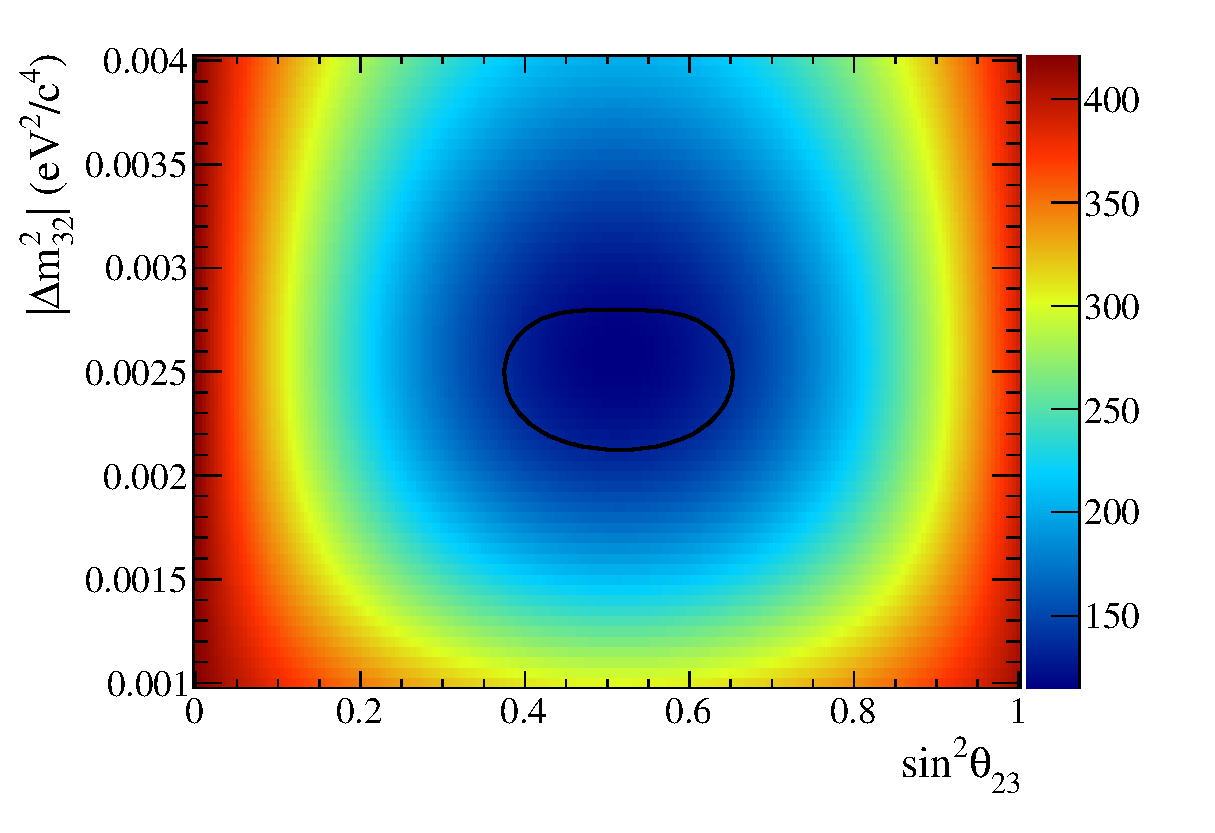
\includegraphics[width=32pc]{./images/spectrum_predictions/nsk_nominalbanff}
\caption {
  Predicted number of 1 $\mu$-like ring events,
  as a function of $\sin^{2}\theta_{23}$ and $|\Delta m^{2}_{32}|$,
  for an exposure of 6.5700$\times$10$^{20}$ POT.
  The numbers of events were calculated using the BANFF-tuned MC templates.
  $\sin^{2}\theta_{13}$, $\sin^{2}\theta_{12}$ and $\Delta m^{2}_{21}$ have the values shown in Tab.\ \ref{tab:pdg2012non23} and $\delta_{CP}$=0.
  The numbers shown were generated assuming the normal hierarchy.
  The T2K Run 1+2+3 90\% C.L.\ region is superimposed for reference.
}
\label{fig:nsk_vs_osc_params_tuned_mc}
\end{figure*}

%...........
%
% spectra, various osc scenarios
%
\begin{figure*}[htb]
\begin{minipage}[t]{0.48\linewidth}
\center
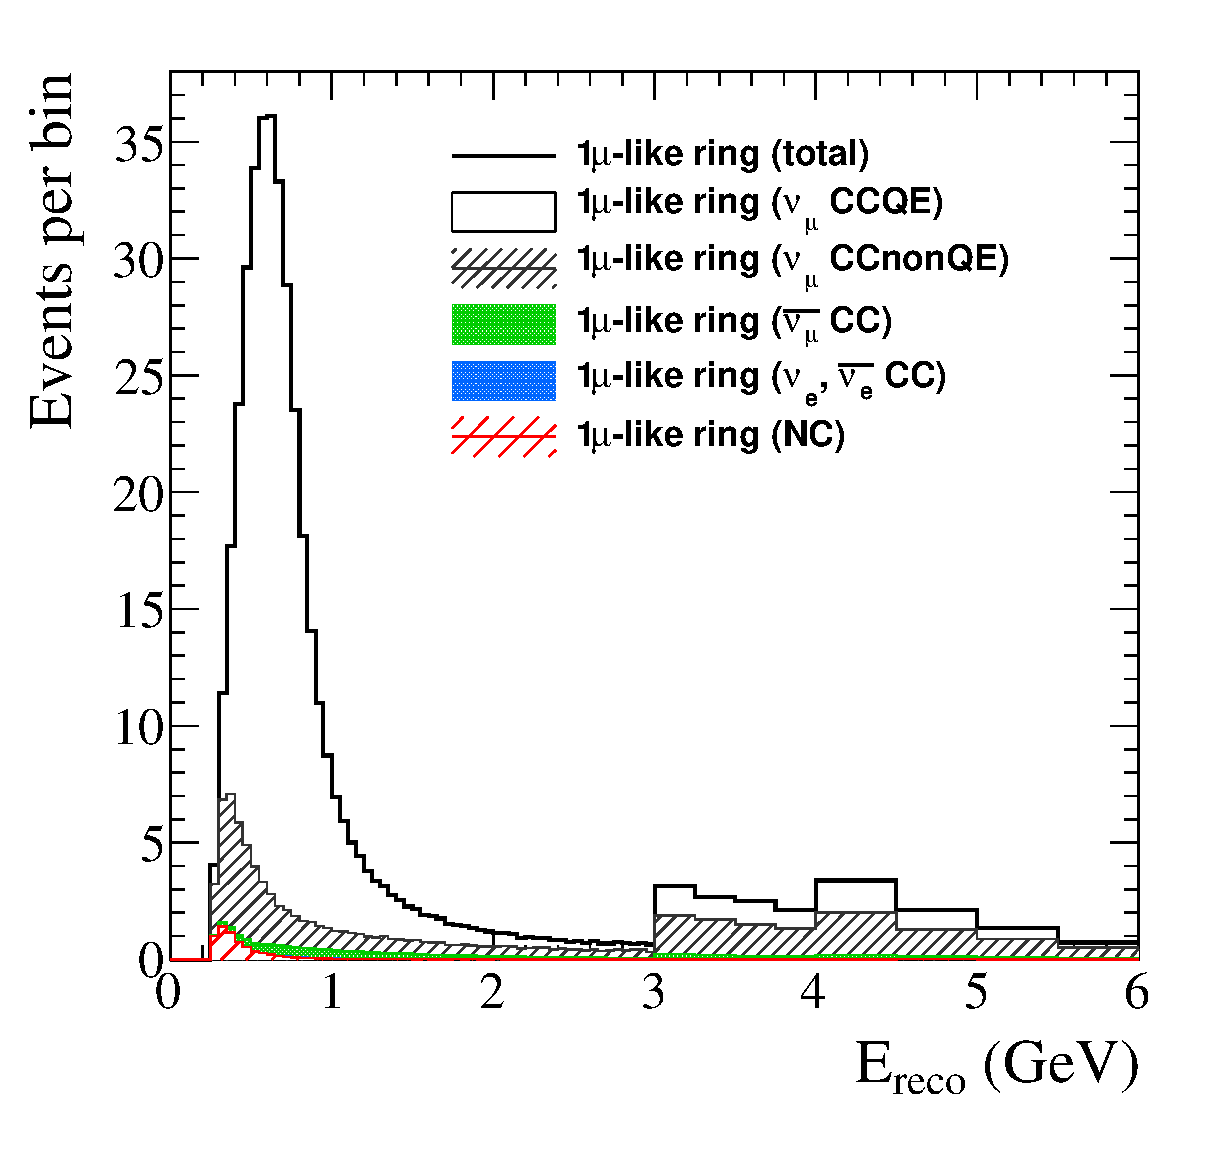
\includegraphics[width=20pc]{./images/spectrum_predictions/spectrum_breakdown_notoscillated_normal}
\caption {
Predicted reconstructed-energy spectrum of 1 $\mu$-like ring events,
and contributions from various true neutrino reaction modes,
for no oscillations and
for an exposure of 6.5700$\times$10$^{20}$ POT.
The 32 components of the spectrum are calculated separately in the actual analysis,
but, for this plot, are grouped into just 5 categories:
$\nu_{\mu}$ CCQE, $\nu_{\mu}$ CCnonQE, $\bar{\nu}_{\mu}$ CC, $\nu_{e}$/$\bar{\nu}_{e}$ CC and NC.
The spectrum was generated using the BANFF-tuned MC templates.
}
\label{fig:1Rmu_spectrum_and_components_no_osc}
\end{minipage}
\hspace{0.06\linewidth}
\begin{minipage}[t]{0.48\linewidth}
\center
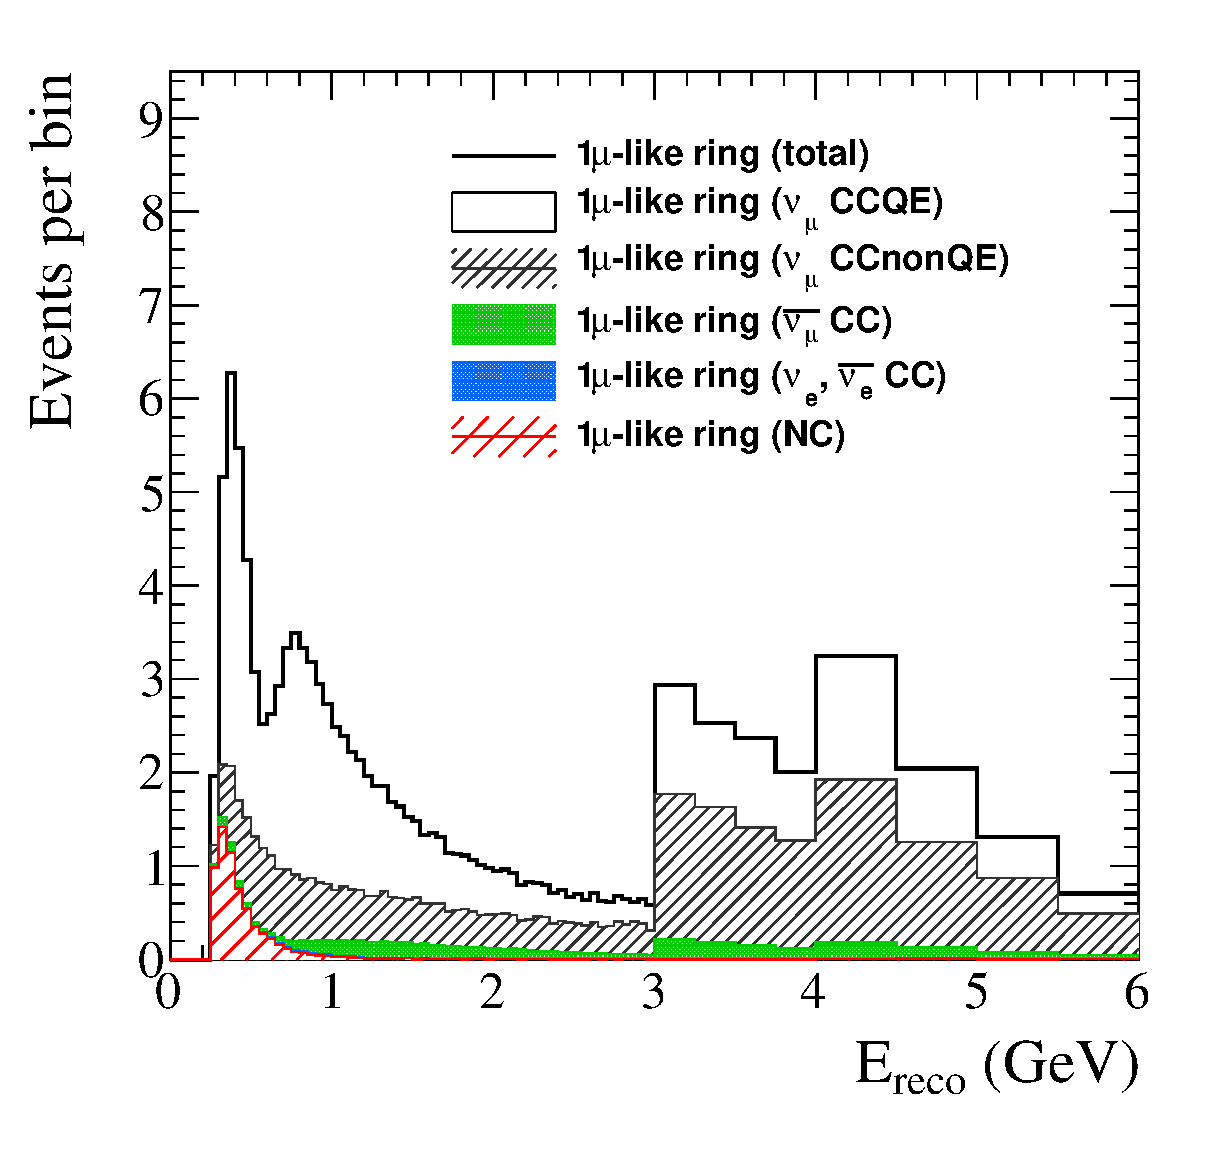
\includegraphics[width=20pc]{./images/spectrum_predictions/spectrum_breakdown_oscillated_normal}
\caption {
Predicted reconstructed-energy spectrum of 1 $\mu$-like ring events,
and contributions from various true neutrino reaction modes,
for oscillations with $\sin^{2}\theta_{23}$=0.5 and $|\Delta m^{2}_{32}|$=2.4$\times10^{-3}$ eV$^{2}$/c$^{4}$
and for an exposure of 6.5700$\times$10$^{20}$ POT.
The spectrum was generated using the BANFF-tuned MC templates.
$\sin^{2}\theta_{13}$, $\sin^{2}\theta_{12}$ and $\Delta m^{2}_{21}$ have the values shown in Tab.\ \ref{tab:pdg2012non23} and $\delta_{CP}$=0.
The spectrum shown was generated assuming the normal hierarchy.
Note that the vertical axis is zoomed in by a factor of 4 compared with Fig.\ \ref{fig:1Rmu_spectrum_and_components_no_osc}.
}
\label{fig:1Rmu_spectrum_and_components_default_osc}
\end{minipage}
\end{figure*}

%...........
%
% effect of tunes on nsk
%
\begin{figure*}[htb]
\begin{minipage}[t]{0.48\linewidth}
\center
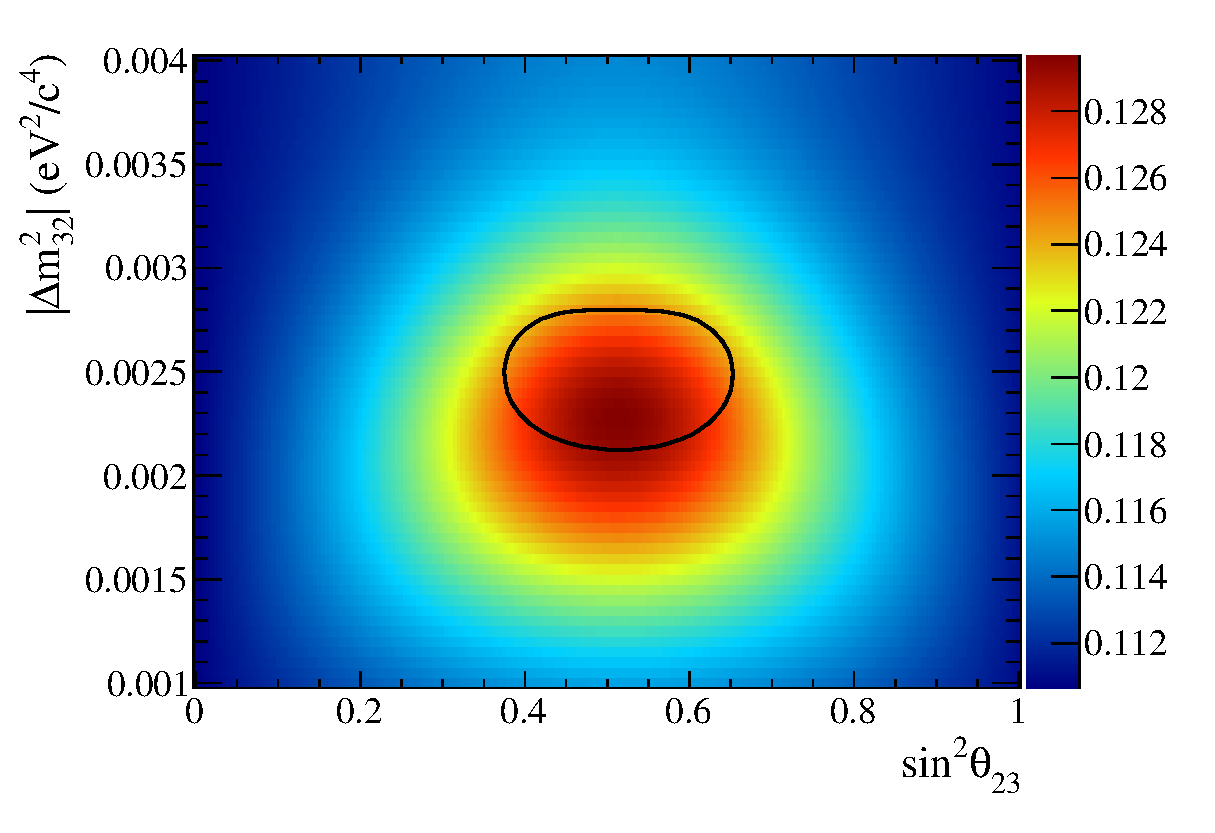
\includegraphics[width=18pc]{./images/spectrum_predictions/nsk_diff_nomflux}
\caption {
  Fractional difference in the predicted number of 1 $\mu$-like ring events
  as a result of applying the NA61 flux tuning to the nominal MC templates.
  These numbers are shown as a function of $\sin^{2}\theta_{23}$ and $|\Delta m^{2}_{32}|$
  for an exposure of 6.5700$\times$10$^{20}$ POT.
  $\sin^{2}\theta_{13}$, $\sin^{2}\theta_{12}$ and $\Delta m^{2}_{21}$ have the values shown in Tab.\ \ref{tab:pdg2012non23} and $\delta_{CP}$=0.
  The numbers shown were generated assuming the normal hierarchy.
  The T2K Run 1+2+3 90\% CL region is superimposed for reference.
}
\label{fig:nsk_vs_osc_params_effect_of_na61_tune}
\end{minipage}
\hspace{0.06\linewidth}
\begin{minipage}[t]{0.48\linewidth}
\center
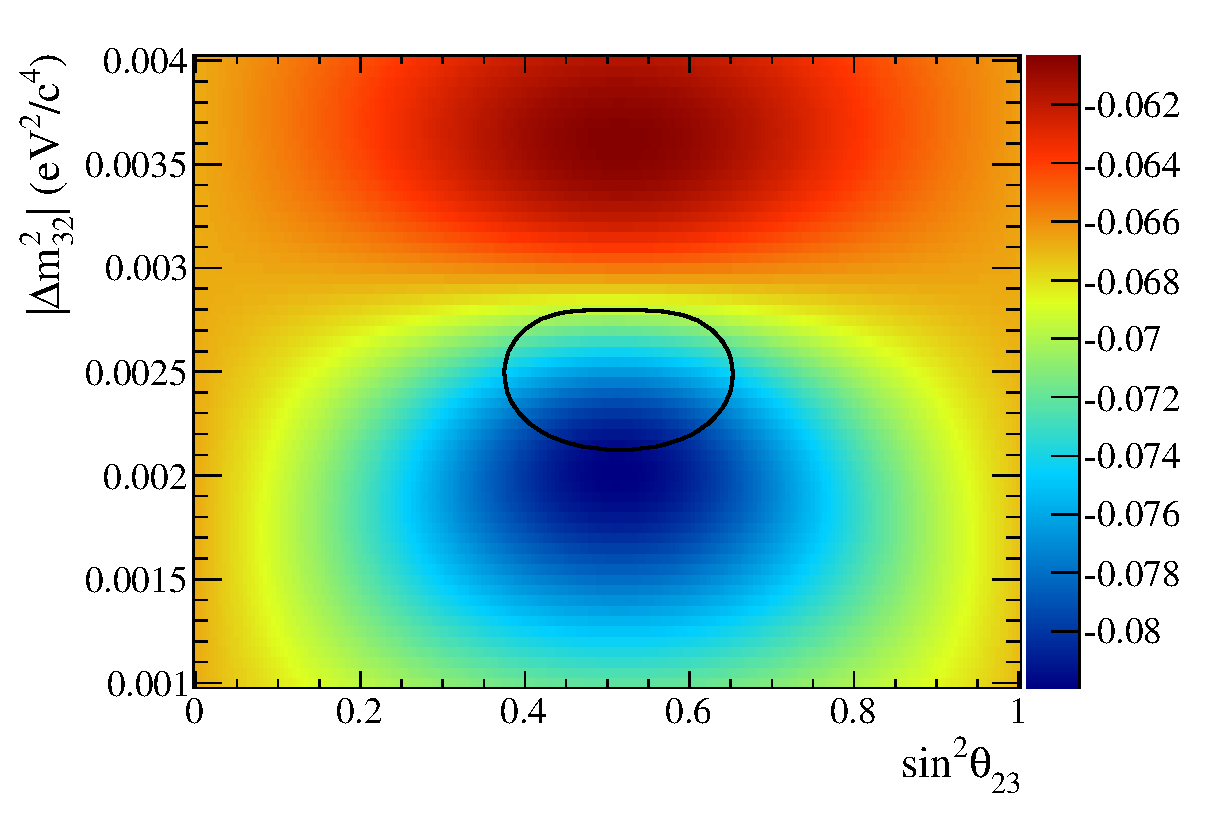
\includegraphics[width=18pc]{./images/spectrum_predictions/nsk_diff_tunflux}
\caption {
  Fractional difference in the predicted number of 1 $\mu$-like ring events
  as a result of applying the BANFF flux and cross-section tuning to the NA61 flux tuned MC templates.
  These numbers are shown as a function of $\sin^{2}\theta_{23}$ and $|\Delta m^{2}_{32}|$ and
  for an exposure of 6.5700$\times$10$^{20}$ POT.
  $\sin^{2}\theta_{13}$, $\sin^{2}\theta_{12}$ and $\Delta m^{2}_{21}$ have the values shown in Tab.\ \ref{tab:pdg2012non23} and $\delta_{CP}$=0.
  The numbers shown were generated assuming the normal hierarchy.
  The T2K Run 1+2+3 90\% CL region is superimposed for reference.
}
\label{fig:nsk_vs_osc_params_effect_of_banff_tune}
\end{minipage}
\end{figure*}

%...........
%
% tables showing the effect of tunes on nsk and nsk components
%

\begin{table}
\centering
\begin{tabular}{| c |  D{.}{.}{-1} |  D{.}{.}{-1} |  D{.}{.}{-1} | }
\hline
         & \multicolumn{1}{c|}{$N_{SK}$}     & \multicolumn{1}{c|}{$N_{SK}$}          & \multicolumn{1}{c|}{$N_{SK}$}          \\ 
         & \multicolumn{1}{c|}{(nominal MC)} & \multicolumn{1}{c|}{(NA61-tuned MC)}  & \multicolumn{1}{c|}{(BANFF-tuned MC)}  \\ 
\hline
Total & 418.131220 & 464.272533 & 445.980111 \\ 
\hline
$\nu_\mu$ CCQE & 332.238749 & 367.166655 & 351.657098 \\ 
$\nu_\mu$ CC 1$\pi$ & 56.190220 & 63.533041 & 62.227879 \\ 
$\nu_\mu$ CC coherent & 1.896444 & 2.136085 & 2.108162 \\ 
$\nu_\mu$ CC other & 7.963009 & 9.600253 & 9.615971 \\ 
$\nu_\mu$/$\nu_\tau$ NC 1$\pi^{+/-}$ & 3.403911 & 3.888131 & 2.934821 \\ 
$\nu_\mu$/$\nu_\tau$ NC other & 2.912186 & 3.428374 & 3.228957 \\ 
Osc. $\nu_\mu$ CCQE & 0.000000 & 0.000000 & 0.000000 \\ 
Osc. $\nu_\mu$ CC 1$\pi$ & 0.000000 & 0.000000 & 0.000000 \\ 
Osc. $\nu_\mu$ CC coherent & 0.000000 & 0.000000 & 0.000000 \\ 
Osc. $\nu_\mu$ CC other & 0.000000 & 0.000000 & 0.000000 \\ 
$\bar{\nu_\mu}$ CCQE & 9.008088 & 9.664244 & 9.521964 \\ 
$\bar{\nu_\mu}$ CC 1$\pi$ & 2.909354 & 3.114170 & 3.061538 \\ 
$\bar{\nu_\mu}$ CC coherent & 0.428081 & 0.458785 & 0.466122 \\ 
$\bar{\nu_\mu}$ CC other & 0.519092 & 0.553722 & 0.548210 \\ 
$\bar{\nu_\mu}$/$\bar{\nu_\tau}$ NC 1$\pi^{+/-}$ & 0.188316 & 0.203257 & 0.143433 \\ 
$\bar{\nu_\mu}$/$\bar{\nu_\tau}$ NC other & 0.176427 & 0.188866 & 0.175090 \\ 
$\nu_e$ CCQE & 0.035370 & 0.038166 & 0.037333 \\ 
$\nu_e$ CC 1$\pi$ & 0.021574 & 0.023840 & 0.023994 \\ 
$\nu_e$ CC coherent & 0.001057 & 0.001158 & 0.001158 \\ 
$\nu_e$ CC other & 0.005812 & 0.006914 & 0.006795 \\ 
$\nu_e$ NC 1$\pi^{+/-}$ & 0.091432 & 0.105093 & 0.075133 \\ 
$\nu_e$ NC other & 0.112184 & 0.131680 & 0.121606 \\ 
$\bar{\nu_e}$ CCQE & 0.002174 & 0.002187 & 0.002102 \\ 
$\bar{\nu_e}$ CC 1$\pi$ & 0.001376 & 0.001385 & 0.001345 \\ 
$\bar{\nu_e}$ CC coherent & 0.000135 & 0.000137 & 0.000137 \\ 
$\bar{\nu_e}$ CC other & 0.000442 & 0.000446 & 0.000432 \\ 
$\bar{\nu_e}$ NC 1$\pi^{+/-}$ & 0.012254 & 0.012354 & 0.008390 \\ 
$\bar{\nu_e}$ NC other & 0.013532 & 0.013592 & 0.012439 \\ 
Osc. $\nu_e$ CCQE & 0.000000 & 0.000000 & 0.000000 \\ 
Osc. $\nu_e$ CC 1$\pi$ & 0.000000 & 0.000000 & 0.000000 \\ 
Osc. $\nu_e$ CC coherent & 0.000000 & 0.000000 & 0.000000 \\ 
Osc. $\nu_e$ CC other & 0.000000 & 0.000000 & 0.000000 \\ 
\hline
\end{tabular}
\caption{
  Calculated numbers of 1-ring $\mu$-like events without oscillations using the nominal MC templates, the
  NA61-tuned MC templates and the BANFF-tuned MC templates.
  The total numbers of events and the numbers of events from each mode considered in this analysis are shown.
  These numbers were calculated for an exposure of 6.5700$\times$10$^{20}$ POT.
}
\label{tab:nsk_nominal_x3_no_osc}
\end{table}


\begin{table}
\centering
\begin{tabular}{| c |  D{.}{.}{-1} |  D{.}{.}{-1} |  D{.}{.}{-1} | }
\hline
         & \multicolumn{1}{c|}{$N_{SK}$}     & \multicolumn{1}{c|}{$N_{SK}$}          & \multicolumn{1}{c|}{$N_{SK}$}          \\ 
         & \multicolumn{1}{c|}{(nominal MC)} & \multicolumn{1}{c|}{(NA61-tuned MC)}  & \multicolumn{1}{c|}{(BANFF-tuned MC)}  \\ 
\hline
Total & 116.283270 & 131.048525 & 124.981851 \\ 
\hline
$\nu_\mu$ CCQE & 66.133875 & 73.447588 & 70.993870 \\ 
$\nu_\mu$ CC 1$\pi$ & 27.733771 & 31.941870 & 29.795498 \\ 
$\nu_\mu$ CC coherent & 0.777452 & 0.896207 & 0.908178 \\ 
$\nu_\mu$ CC other & 7.072249 & 8.586001 & 8.597815 \\ 
$\nu_\mu$/$\nu_\tau$ NC 1$\pi^{+/-}$ & 3.403911 & 3.888131 & 2.934821 \\ 
$\nu_\mu$/$\nu_\tau$ NC other & 2.912186 & 3.428374 & 3.228957 \\ 
Osc. $\nu_\mu$ CCQE & 0.117417 & 0.129898 & 0.127451 \\ 
Osc. $\nu_\mu$ CC 1$\pi$ & 0.027388 & 0.030497 & 0.030950 \\ 
Osc. $\nu_\mu$ CC coherent & 0.000821 & 0.000913 & 0.000913 \\ 
Osc. $\nu_\mu$ CC other & 0.002344 & 0.002648 & 0.002609 \\ 
$\bar{\nu_\mu}$ CCQE & 4.428977 & 4.745506 & 4.621408 \\ 
$\bar{\nu_\mu}$ CC 1$\pi$ & 2.080140 & 2.219962 & 2.132869 \\ 
$\bar{\nu_\mu}$ CC coherent & 0.228753 & 0.244521 & 0.248227 \\ 
$\bar{\nu_\mu}$ CC other & 0.460554 & 0.490899 & 0.485509 \\ 
$\bar{\nu_\mu}$/$\bar{\nu_\tau}$ NC 1$\pi^{+/-}$ & 0.188316 & 0.203257 & 0.143433 \\ 
$\bar{\nu_\mu}$/$\bar{\nu_\tau}$ NC other & 0.176427 & 0.188866 & 0.175090 \\ 
$\nu_e$ CCQE & 0.032854 & 0.035470 & 0.034683 \\ 
$\nu_e$ CC 1$\pi$ & 0.020475 & 0.022660 & 0.022716 \\ 
$\nu_e$ CC coherent & 0.000987 & 0.001084 & 0.001084 \\ 
$\nu_e$ CC other & 0.005716 & 0.006807 & 0.006690 \\ 
$\nu_e$ NC 1$\pi^{+/-}$ & 0.091432 & 0.105093 & 0.075133 \\ 
$\nu_e$ NC other & 0.112184 & 0.131680 & 0.121606 \\ 
$\bar{\nu_e}$ CCQE & 0.002085 & 0.002096 & 0.002014 \\ 
$\bar{\nu_e}$ CC 1$\pi$ & 0.001337 & 0.001345 & 0.001303 \\ 
$\bar{\nu_e}$ CC coherent & 0.000130 & 0.000132 & 0.000132 \\ 
$\bar{\nu_e}$ CC other & 0.000438 & 0.000442 & 0.000429 \\ 
$\bar{\nu_e}$ NC 1$\pi^{+/-}$ & 0.012254 & 0.012354 & 0.008390 \\ 
$\bar{\nu_e}$ NC other & 0.013532 & 0.013592 & 0.012439 \\ 
Osc. $\nu_e$ CCQE & 0.179722 & 0.198093 & 0.190000 \\ 
Osc. $\nu_e$ CC 1$\pi$ & 0.059387 & 0.065728 & 0.070982 \\ 
Osc. $\nu_e$ CC coherent & 0.004749 & 0.005234 & 0.005093 \\ 
Osc. $\nu_e$ CC other & 0.001406 & 0.001578 & 0.001558 \\ 
\hline
\end{tabular}
\caption{
Calculated numbers of 1-ring $\mu$-like events using the nominal MC templates, the NA61-tuned MC templates
and the BANFF-tuned MC templates.
The total numbers of events and the numbers of events from each mode considered in this analysis are shown.
These numbers were calculated for an exposure of 6.5700$\times$10$^{20}$ POT
and oscillations with $\sin^{2}\theta_{23}$=0.5 and $|\Delta m^{2}_{32}|$=2.4$\times$10$^{-3}$ eV$^{2}$/c$^{4}$.
Values shown in Tab. \ref{tab:pdg2012non23} are used for $\sin^{2}\theta_{13}$, $\sin^{2}\theta_{12}$ and $\Delta m^{2}_{21}$ and $\delta_{CP}$=0.
The normal mass hierarchy is assumed.
}
\label{tab:nsk_nominal_x3_default_osc}
\end{table}


%...........
%
% Plots showing the effect of tunes on Ereco spectra
%
\begin{figure*}[htb]
\center
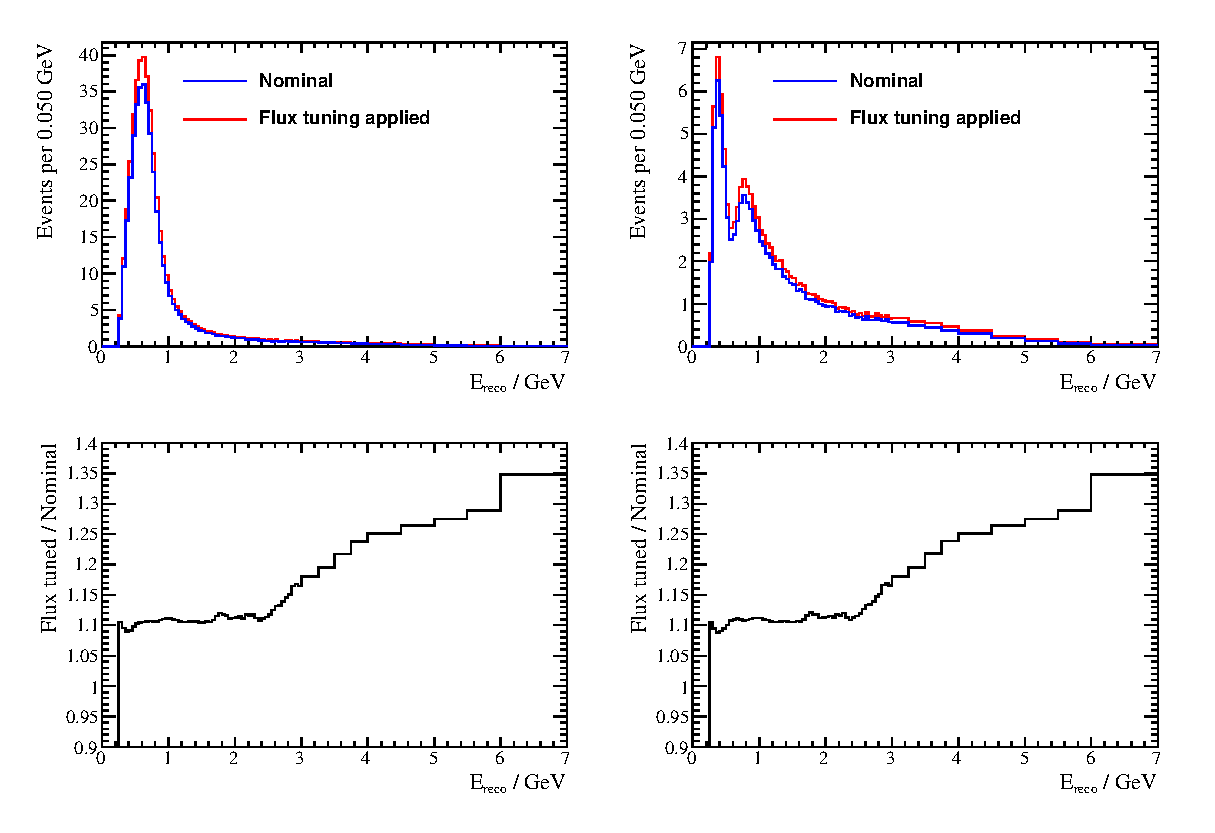
\includegraphics[width=30pc]{./images/spectrum_predictions/spectra_nom_fluxtuned}
\caption {
Top: Reconstructed-energy spectrum of 1 $\mu$-like ring events,
for an exposure of 6.5700$\times$10$^{20}$ POT,
both with and without the effect of the NA61 flux tuning of the nominal MC templates.
The spectra are shown both for no oscillations (left)
and for oscillations with $\sin^{2}\theta_{23}$=0.5, $|\Delta m^{2}_{32}|$=2.4$\times$10$^{-3}$ eV$^{2}$/c$^{4}$,
the 2012 PDG values for $\sin^{2}\theta_{13}$, $\sin^{2}\theta_{12}$ and $\Delta m^{2}_{21}$, and
$\delta_{CP}$=0 (right). Results shown for the normal hierarchy.
Bottom: Ratio of flux-tuned spectrum to the nominal MC spectrum.
}
\label{fig:1Rmu_spectrum_w_and_wo_na61_weights}
\end{figure*}

\begin{figure*}[htb]
\center
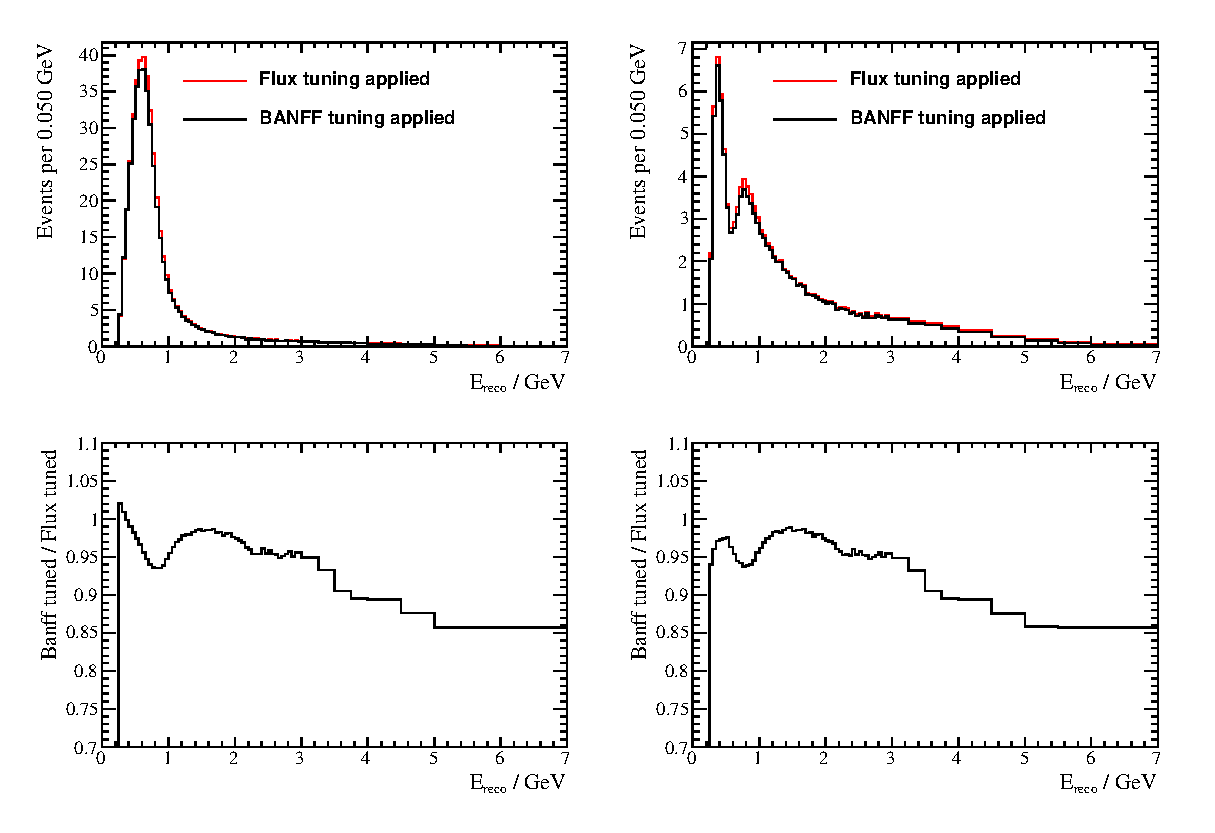
\includegraphics[width=30pc]{./images/spectrum_predictions/spectra_tun_banfftuned}
\caption {
Top: Reconstructed-energy spectrum of 1 $\mu$-like ring events,
for an exposure of 6.5700$\times$10$^{20}$ POT,
both with and without the effect of BANFF flux and cross-section tuning on the NA61-tuned flux MC templates.
The spectra are shown both for no 23-sector oscillations (left)
and for oscillations with $\sin^{2}\theta_{23}$=0.5 and $|\Delta m^{2}_{32}|$=2.4$\times$10$^{-3}$ eV$^{2}$/c$^{4}$ (right).
In all spectra, the 2012 PDG parameters are used for $\sin^{2}\theta_{13}$, $\sin^{2}\theta_{12}$ and $\Delta m^{2}_{21}$
and $\delta_{CP}$=0. Results shown for the normal hierarchy.
Bottom: Ratio of BANFF-tuned spectrum to the flux-tuned spectrum.
}
\label{fig:1Rmu_spectrum_w_and_wo_banff_weights}
\end{figure*}

